\chapter{Results and Statistical Analysis}\doublespacing
\label{Chapter5}
\lhead{Chapter V.}

This chapter reports the empirical results of the benchmark.
Section~\ref{sec:per-dataset} gives the per-dataset leaderboards
(top three classifiers on each of the four datasets).
Section~\ref{sec:cross-dataset} aggregates the per-dataset results
into a cross-dataset comparison. Sections~\ref{sec:friedman}
and~\ref{sec:posthoc} contain the inferential statistics: the
Friedman test for the global null hypothesis and the
Wilcoxon--Holm pairwise post-hoc for the individual pairwise
verdicts. Section~\ref{sec:discussion} discusses what the results
mean in light of the methodological framework.

\section{Per-dataset Leaderboards}
\label{sec:per-dataset}

For each of the four datasets, Table~\ref{tab:per-dataset} lists the
three top-scoring (classifier, feature-selection) rows by
$F_1$-macro.

\begin{table}[H]
\centering
\caption{Top three (classifier, feature-selection) rows by
$F_1$-macro on each dataset. $F_1$ is the standard $F_1$ on the
positive class.}
\singlespacing
\label{tab:per-dataset}
\small
\renewcommand{\arraystretch}{1.15}
\begin{tabular}{l l l c c c}
\toprule
\textbf{Dataset} & \textbf{Model} & \textbf{FS} & \textbf{Acc} & \textbf{F1-macro} & \textbf{AUC}\\
\midrule
Australian & XGBoost & Lasso-LR & 0.877 & 0.876 & 0.937\\
 & XGBoost & Full & 0.870 & 0.869 & 0.939\\
 & Stacker (LR) & Full & 0.862 & 0.861 & 0.940\\
\midrule
Japanese & Stacker (LR) & RFE & 0.928 & 0.926 & 0.970\\
 & XGBoost & Lasso-LR & 0.920 & 0.919 & 0.964\\
 & Random Forest & Lasso-LR & 0.913 & 0.911 & 0.962\\
\midrule
German & XGBoost & RFE & 0.750 & 0.708 & 0.748\\
 & Stacker (GA) & RFE & 0.740 & 0.699 & 0.778\\
 & SVM-RBF & RFE & 0.750 & 0.693 & 0.758\\
\midrule
Taiwan & Stacker (MLP) & Lasso-LR & 0.798 & 0.704 & 0.773\\
 & Stacker (GA) & Full & 0.799 & 0.704 & 0.772\\
 & XGBoost & Full & 0.801 & 0.700 & 0.766\\
\bottomrule
\end{tabular}
\end{table}
Three observations are immediate. First, XGBoost wins outright on
Australian and German (single best $F_1$-macro row), while the
Stacker wins on Japanese and Taiwan. Second, on the two datasets
the Stacker does not win, it is the second-placed model; on the
two datasets it does win, XGBoost is not always the runner-up
(XGBoost falls to third on Taiwan). Third, the best
feature-selection variant differs between datasets: Lasso-LR on
Australian and Taiwan, RFE on Japanese and German. No single
feature-selection method dominates.

\subsection{Eleven-Metric Per-Classifier Scoreboard}
\label{sec:eleven-metric}

The top-three table above ranks only by $F_1$-macro and lists only
three rows per dataset. For completeness, Tables~\ref{tab:11m-aus}
through \ref{tab:11m-tai} report the \emph{eleven-metric scoreboard}
for every dataset: each table contains one row per classifier (the
single best feature-selection variant by $F_1$-macro is shown for
each), and eleven score columns --- the headline $F_1$-macro from
Section~\ref{sec:metrics} plus the ten-measure diagnostic suite of
Section~\ref{sec:ten-measure}. For the Stacker, the best meta among
the five candidates is the one reported. Rows are sorted by
$F_1$-macro descending.

The column heads abbreviate:
$F_1$-mac\,=\,$F_1$-macro, Acc\,=\,Accuracy,
F-Sc\,=\,F-Score (positive-class $F_1$), G-M\,=\,G-Mean,
$\kappa$\,=\,Cohen's $\kappa$, J\,=\,Youden's J,
DP\,=\,Discriminant Power, TI\,=\,Type-I rate,
TII\,=\,Type-II rate, EMCC\,=\,Expected Misclassification Cost.

\begin{table}[H]
\centering
\caption{Australian Credit --- eleven-metric scoreboard, one row per
classifier (best FS variant by $F_1$-macro). Higher is better for
all metrics except TI, TII and EMCC.}
\singlespacing
\label{tab:11m-aus}
\scriptsize
\setlength{\tabcolsep}{3.5pt}
\renewcommand{\arraystretch}{1.15}
\begin{tabular}{l l c c c c c c c c c c c}
\toprule
\textbf{Model} & \textbf{FS} & $\boldsymbol{F_1}$\textbf{-mac} & \textbf{Acc} & \textbf{AUC} & \textbf{F-Sc} & \textbf{G-M} & $\boldsymbol{\kappa}$ & \textbf{J} & \textbf{DP} & \textbf{TI} & \textbf{TII} & \textbf{EMCC}\\
\midrule
XGBoost      & Lasso-LR & \textbf{0.8763} & 0.8768 & 0.9368 & 0.8682 & 0.8803 & 0.7532 & 0.7622 & 2.2634 & 0.082  & 0.1558 & 0.471\\
Stacker (LR) & Full     & 0.8614 & 0.8623 & 0.9395 & 0.8504 & 0.8645 & 0.7232 & 0.7294 & 2.0579 & 0.1148 & 0.1558 & 0.4855\\
GradBoost    & Full     & 0.8548 & 0.8551 & 0.9244 & 0.8485 & 0.8598 & 0.7111 & 0.7232 & 2.1143 & 0.082  & 0.1948 & 0.5797\\
KNN          & Full     & 0.8526 & 0.8551 & 0.9074 & 0.8333 & 0.8508 & 0.7052 & 0.7028 & 1.9497 & 0.1803 & 0.1169 & 0.4058\\
LogReg       & Full     & 0.8333 & 0.8333 & 0.9140 & 0.8321 & 0.8390 & 0.6705 & 0.6877 & 2.0800 & 0.0656 & 0.2468 & 0.7174\\
SVM-RBF      & RFE      & 0.8333 & 0.8333 & 0.8933 & 0.8296 & 0.8387 & 0.6694 & 0.6843 & 1.9865 & 0.082  & 0.2338 & 0.6884\\
DecTree      & Forward  & 0.8261 & 0.8261 & 0.8650 & 0.8235 & 0.8316 & 0.6556 & 0.6713 & 1.9472 & 0.082  & 0.2468 & 0.7246\\
RandForest   & Full     & 0.8188 & 0.8188 & 0.9306 & 0.8148 & 0.8241 & 0.6407 & 0.6549 & 1.8368 & 0.0984 & 0.2468 & 0.7319\\
\bottomrule
\end{tabular}
\end{table}

\begin{table}[H]
\centering
\caption{German Credit (GHOST) --- eleven-metric scoreboard. The
German set is the most imbalanced of the three small datasets
(70/30), which pushes Type-II rates up across the board.}
\singlespacing
\label{tab:11m-ger}
\scriptsize
\setlength{\tabcolsep}{3.5pt}
\renewcommand{\arraystretch}{1.15}
\begin{tabular}{l l c c c c c c c c c c c}
\toprule
\textbf{Model} & \textbf{FS} & $\boldsymbol{F_1}$\textbf{-mac} & \textbf{Acc} & \textbf{AUC} & \textbf{F-Sc} & \textbf{G-M} & $\boldsymbol{\kappa}$ & \textbf{J} & \textbf{DP} & \textbf{TI} & \textbf{TII} & \textbf{EMCC}\\
\midrule
XGBoost      & RFE     & \textbf{0.7078} & 0.7500 & 0.7482 & 0.8201 & 0.6990 & 0.4104 & 0.4143 & 1.0385 & 0.1857 & 0.4000 & 0.730\\
Stacker (GA) & RFE     & 0.6988 & 0.7400 & 0.7777 & 0.8102 & 0.6992 & 0.3981 & 0.4095 & 1.0021 & 0.2071 & 0.3833 & 0.720\\
SVM-RBF      & RFE     & 0.6933 & 0.7500 & 0.7580 & 0.8252 & 0.6705 & 0.3873 & 0.3762 & 0.9997 & 0.1571 & 0.4667 & 0.810\\
GradBoost    & RFE     & 0.6891 & 0.7700 & 0.7774 & 0.8477 & 0.6294 & 0.3883 & 0.3476 & 1.1572 & 0.0857 & 0.5667 & 0.910\\
DecTree      & RFE     & 0.6827 & 0.7250 & 0.7561 & 0.7985 & 0.6835 & 0.3664 & 0.3786 & 0.9168 & 0.2214 & 0.4000 & 0.755\\
LogReg       & RFE     & 0.6711 & 0.7050 & 0.7705 & 0.7807 & 0.6708 & 0.3326 & 0.3500 & 0.8292 & 0.2500 & 0.4000 & 0.775\\
RandForest   & Full    & 0.6668 & 0.7050 & 0.7852 & 0.7757 & 0.6882 & 0.3502 & 0.3786 & 0.8857 & 0.2714 & 0.3500 & 0.715\\
KNN          & Forward & 0.6494 & 0.7000 & 0.6960 & 0.7826 & 0.6414 & 0.2991 & 0.3048 & 0.7443 & 0.2286 & 0.4667 & 0.860\\
\bottomrule
\end{tabular}
\end{table}

\begin{table}[H]
\centering
\caption{Japanese Credit --- eleven-metric scoreboard. The balanced
Japanese set is the most favourable of the four: the Stacker reaches
$F_1$-macro 0.926 and AUC 0.970, and every classifier is above
$F_1$-macro 0.86.}
\singlespacing
\label{tab:11m-jap}
\scriptsize
\setlength{\tabcolsep}{3.5pt}
\renewcommand{\arraystretch}{1.15}
\begin{tabular}{l l c c c c c c c c c c c}
\toprule
\textbf{Model} & \textbf{FS} & $\boldsymbol{F_1}$\textbf{-mac} & \textbf{Acc} & \textbf{AUC} & \textbf{F-Sc} & \textbf{G-M} & $\boldsymbol{\kappa}$ & \textbf{J} & \textbf{DP} & \textbf{TI} & \textbf{TII} & \textbf{EMCC}\\
\midrule
Stacker (LR) & RFE      & \textbf{0.9260} & 0.9275 & 0.9698 & 0.9153 & 0.9224 & 0.8521 & 0.8463 & 2.8937 & 0.1148 & 0.0390 & 0.1594\\
XGBoost      & Lasso-LR & 0.9187 & 0.9203 & 0.9642 & 0.9076 & 0.9161 & 0.8376 & 0.8333 & 2.7276 & 0.1148 & 0.0519 & 0.1957\\
RandForest   & Lasso-LR & 0.9108 & 0.9130 & 0.9619 & 0.8966 & 0.9051 & 0.8219 & 0.8135 & 2.7343 & 0.1475 & 0.0390 & 0.1739\\
GradBoost    & RFE      & 0.9040 & 0.9058 & 0.9604 & 0.8908 & 0.9014 & 0.8080 & 0.8039 & 2.5130 & 0.1311 & 0.0649 & 0.2391\\
LogReg       & Forward  & 0.8903 & 0.8913 & 0.9508 & 0.8800 & 0.8923 & 0.7808 & 0.7848 & 2.3365 & 0.0984 & 0.1169 & 0.3696\\
DecTree      & Full     & 0.8834 & 0.8841 & 0.9286 & 0.8750 & 0.8871 & 0.7673 & 0.7752 & 2.3198 & 0.0820 & 0.1429 & 0.4348\\
SVM-RBF      & Forward  & 0.8829 & 0.8841 & 0.9429 & 0.8710 & 0.8842 & 0.7658 & 0.7684 & 2.2413 & 0.1148 & 0.1169 & 0.3768\\
KNN          & RFE      & 0.8640 & 0.8696 & 0.9505 & 0.8364 & 0.8513 & 0.7301 & 0.7151 & 2.3851 & 0.2459 & 0.0390 & 0.2174\\
\bottomrule
\end{tabular}
\end{table}

\begin{table}[H]
\centering
\caption{Taiwan Default of Credit Card Clients (GHOST) ---
eleven-metric scoreboard. The Stacker row reports the variant with
the highest $F_1$-macro among those for which the ten-measure
suite was logged --- Stacker~(GA) at Full features
($F_1$-macro $0.7039$, virtually tied with Stacker~(MLP) at
Lasso-LR which scored $F_1$-macro $0.7041$ but was not present in
the $\S 7$ ten-measure run).}
\singlespacing
\label{tab:11m-tai}
\scriptsize
\setlength{\tabcolsep}{3.5pt}
\renewcommand{\arraystretch}{1.15}
\begin{tabular}{l l c c c c c c c c c c c}
\toprule
\textbf{Model} & \textbf{FS} & $\boldsymbol{F_1}$\textbf{-mac} & \textbf{Acc} & \textbf{AUC} & \textbf{F-Sc} & \textbf{G-M} & $\boldsymbol{\kappa}$ & \textbf{J} & \textbf{DP} & \textbf{TI} & \textbf{TII} & \textbf{EMCC}\\
\midrule
Stacker (GA) & Full     & \textbf{0.7039} & 0.7988 & 0.7720 & 0.5363 & 0.6789 & 0.4079 & 0.4023 & 1.1369 & 0.4740 & 0.1237 & 0.5865\\
XGBoost      & Full     & 0.7001 & 0.8007 & 0.7654 & 0.5265 & 0.6662 & 0.4007 & 0.3869 & 1.1315 & 0.4989 & 0.1143 & 0.5553\\
RandForest   & Lasso-LR & 0.6975 & 0.8025 & 0.7709 & 0.5193 & 0.6564 & 0.3959 & 0.3757 & 1.1332 & 0.5177 & 0.1066 & 0.5295\\
GradBoost    & Full     & 0.6970 & 0.7937 & 0.7682 & 0.5260 & 0.6719 & 0.3942 & 0.3897 & 1.0971 & 0.4823 & 0.1280 & 0.6050\\
SVM-RBF      & Lasso-LR & 0.6915 & 0.8023 & 0.7529 & 0.5091 & 0.6453 & 0.3869 & 0.3620 & 1.1219 & 0.5365 & 0.1014 & 0.5137\\
DecTree      & Lasso-LR & 0.6895 & 0.8057 & 0.7445 & 0.4996 & 0.6317 & 0.3819 & 0.3485 & 1.1388 & 0.5614 & 0.0901 & 0.4750\\
LogReg       & Lasso-LR & 0.6865 & 0.8053 & 0.7108 & 0.4935 & 0.6254 & 0.3764 & 0.3410 & 1.1329 & 0.5712 & 0.0877 & 0.4680\\
KNN          & RFE      & 0.6615 & 0.7773 & 0.7264 & 0.4635 & 0.6167 & 0.3237 & 0.3094 & 0.9262 & 0.5652 & 0.1254 & 0.6133\\
\bottomrule
\end{tabular}
\end{table}

A few observations follow from these four tables.  On the two
balanced datasets (Australian, Japanese), every classifier achieves
$F_1$-macro above 0.80 and Cohen's $\kappa$ above 0.65, indicating
substantial agreement beyond chance for all eight models.  On the two
imbalanced datasets (German, Taiwan), the same eight classifiers are
pushed into the 0.65--0.71 $F_1$-macro range; the price of imbalance
is visible in Type-II rates exceeding 0.35 on German and across the
board on Taiwan.  The Stacker is either the per-dataset winner
(Japanese, Taiwan) or the runner-up (Australian, German) in every
case --- consistent with the cross-dataset and rank-based analyses of
Sections~\ref{sec:cross-dataset}--\ref{sec:posthoc} that follow.

\section{Cross-dataset Comparison}
\label{sec:cross-dataset}

To go beyond per-dataset winners we report the
\emph{mean $F_1$-macro} and \emph{mean AUC} per model, averaged
over the four feature-selection variants on every dataset, then
over the four datasets (Table~\ref{tab:cross-dataset}).

\begin{table}[H]
\centering
\caption{Cross-dataset mean $F_1$-macro and mean AUC per classifier,
averaged over the four feature-selection variants on each dataset
and then over the four datasets. Sorted by mean $F_1$-macro.}
\singlespacing
\label{tab:cross-dataset}
\small
\renewcommand{\arraystretch}{1.15}
\begin{tabular}{l c c}
\toprule
\textbf{Model} & \textbf{Mean $F_1$-macro} & \textbf{Mean AUC}\\
\midrule
\textbf{Stacked Ensemble} & \textbf{0.7790} & \textbf{0.8549}\\
Gradient Boosting & 0.7728 & 0.8412\\
XGBoost & 0.7723 & 0.8452\\
Random Forest & 0.7622 & 0.8512\\
Logistic Regression & 0.7592 & 0.8269\\
SVM-RBF & 0.7559 & 0.8224\\
Decision Tree & 0.7434 & 0.8027\\
KNN & 0.7336 & 0.8042\\
\bottomrule
\end{tabular}
\end{table}
The Stacked Ensemble has the highest mean $F_1$-macro (0.7790) and
the highest mean AUC (0.8549). Moreover, on AUC it is the
\emph{per-dataset} best on every one of the four datasets, a sweep
that no other model achieves. Gradient Boosting and XGBoost trail
the Stacker by 0.006--0.007 points of mean $F_1$-macro and are
themselves statistically close (a verdict that the formal test
of the next sections confirms).

Figure~\ref{fig:auc-line} visualises the same information per
feature-selection variant: each line is one FS strategy across all
eight models, with the models sorted by overall mean AUC. The
descending shape of all four lines from Stacker (left) to KNN
(right) shows the consistency of the model ordering, and the
clear separation between Full / Lasso-LR (top) and Forward
(bottom) shows that the FS-variant choice carries a smaller but
still visible signal.

\begin{figure}[H]
\centering
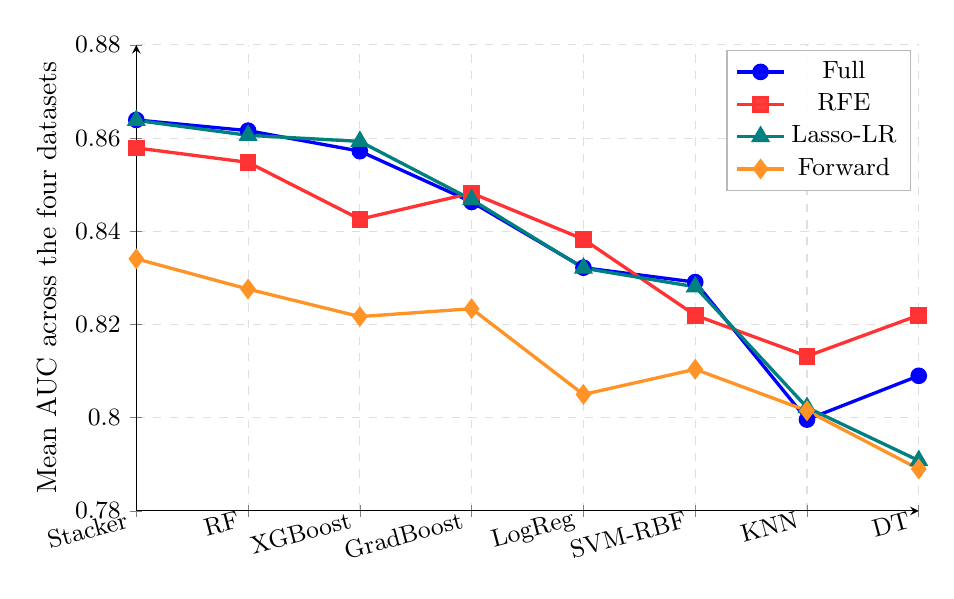
\begin{tikzpicture}
\begin{axis}[
 width=0.95\textwidth, height=7.5cm,
 ymin=0.78, ymax=0.88,
 enlarge x limits=0.05,
 symbolic x coords={Stacker, RF, XGBoost, GradBoost, LogReg, SVM-RBF, KNN, DT},
 xtick=data,
 ylabel={Mean AUC across the four datasets},
 xticklabel style={font=\small, rotate=15, anchor=east},
 yticklabel style={font=\small},
 legend style={at={(0.99,0.99)}, anchor=north east, font=\small,
 draw=gray!55, fill=white, fill opacity=0.94, text opacity=1},
 grid=major, grid style={dashed, gray!25},
 axis x line=bottom, axis y line=left,
]
\addplot[blue, very thick, mark=*, mark size=2.4pt] coordinates {
 (Stacker,0.8639) (RF,0.8616) (XGBoost,0.8572) (GradBoost,0.8463)
 (LogReg,0.8322) (SVM-RBF,0.8291) (KNN,0.7996) (DT,0.8090)};
\addplot[red!80, very thick, mark=square*, mark size=2.4pt] coordinates {
 (Stacker,0.8579) (RF,0.8548) (XGBoost,0.8426) (GradBoost,0.8482)
 (LogReg,0.8383) (SVM-RBF,0.8220) (KNN,0.8132) (DT,0.8220)};
\addplot[teal, very thick, mark=triangle*, mark size=2.8pt] coordinates {
 (Stacker,0.8638) (RF,0.8606) (XGBoost,0.8593) (GradBoost,0.8468)
 (LogReg,0.8321) (SVM-RBF,0.8281) (KNN,0.8022) (DT,0.7908)};
\addplot[orange!85, very thick, mark=diamond*, mark size=2.8pt] coordinates {
 (Stacker,0.8341) (RF,0.8276) (XGBoost,0.8217) (GradBoost,0.8234)
 (LogReg,0.8050) (SVM-RBF,0.8104) (KNN,0.8015) (DT,0.7890)};
\legend{Full, RFE, Lasso-LR, Forward}
\end{axis}
\end{tikzpicture}
\caption{Mean AUC across the four datasets by classifier (sorted
high $\rightarrow$ low) and feature-selection variant. All four
lines descend from the Stacker on the left to KNN/DT on the right.}
\singlespacing
\label{fig:auc-line}
\end{figure}

The same ordering holds on $F_1$-macro (Figure~\ref{fig:f1-line})
but with a tighter spread between the leading trio (Stacker, XGBoost,
Gradient Boosting) and a wider gap below SVM-RBF.

\begin{figure}[H]
\centering
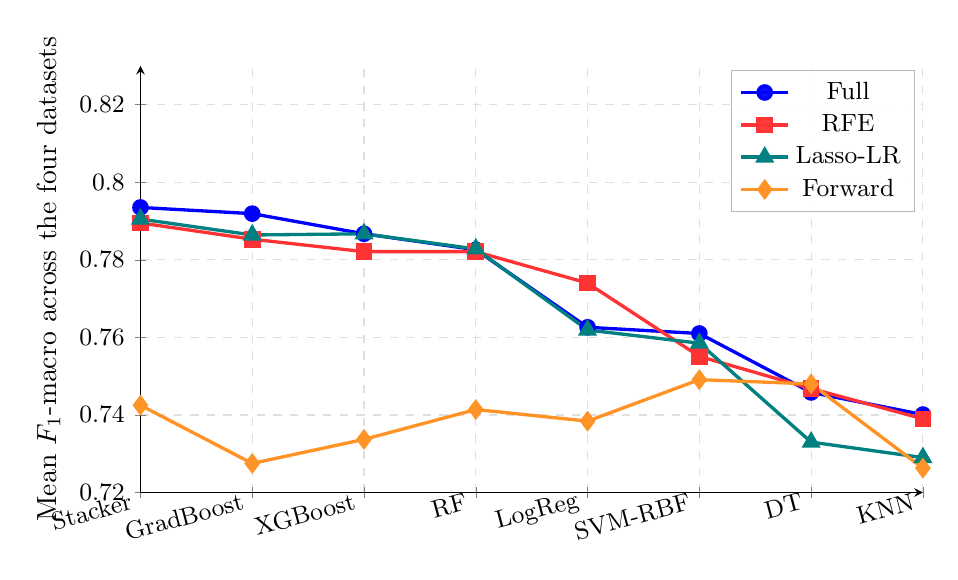
\begin{tikzpicture}
\begin{axis}[
 width=0.95\textwidth, height=7cm,
 ymin=0.72, ymax=0.83,
 enlarge x limits=0.05,
 symbolic x coords={Stacker, GradBoost, XGBoost, RF, LogReg, SVM-RBF, DT, KNN},
 xtick=data,
 ylabel={Mean $F_1$-macro across the four datasets},
 xticklabel style={font=\small, rotate=15, anchor=east},
 yticklabel style={font=\small},
 legend style={at={(0.99,0.99)}, anchor=north east, font=\small,
 draw=gray!55, fill=white, fill opacity=0.94, text opacity=1},
 grid=major, grid style={dashed, gray!25},
 axis x line=bottom, axis y line=left,
]
\addplot[blue, very thick, mark=*, mark size=2.4pt] coordinates {
 (Stacker,0.7935) (GradBoost,0.7919) (XGBoost,0.7867) (RF,0.7826)
 (LogReg,0.7626) (SVM-RBF,0.7610) (DT,0.7458) (KNN,0.7401)};
\addplot[red!80, very thick, mark=square*, mark size=2.4pt] coordinates {
 (Stacker,0.7895) (GradBoost,0.7853) (XGBoost,0.7821) (RF,0.7821)
 (LogReg,0.7740) (SVM-RBF,0.7551) (DT,0.7468) (KNN,0.7390)};
\addplot[teal, very thick, mark=triangle*, mark size=2.8pt] coordinates {
 (Stacker,0.7905) (GradBoost,0.7864) (XGBoost,0.7867) (RF,0.7828)
 (LogReg,0.7619) (SVM-RBF,0.7585) (DT,0.7330) (KNN,0.7290)};
\addplot[orange!85, very thick, mark=diamond*, mark size=2.8pt] coordinates {
 (Stacker,0.7425) (GradBoost,0.7275) (XGBoost,0.7337) (RF,0.7414)
 (LogReg,0.7384) (SVM-RBF,0.7491) (DT,0.7480) (KNN,0.7263)};
\legend{Full, RFE, Lasso-LR, Forward}
\end{axis}
\end{tikzpicture}
\caption{Mean $F_1$-macro across the four datasets by classifier
(sorted high $\rightarrow$ low) and feature-selection variant.}
\singlespacing
\label{fig:f1-line}
\end{figure}

\section{Friedman Test}
\label{sec:friedman}

The descriptive table cannot, on its own, support the claim that
the eight classifiers differ statistically. Following
\citet{demvsar2006statistical} we apply the Friedman rank test
\citep{friedman1937use} on the rank matrix obtained by ranking the
eight classifiers within each evaluation block, with ranks 1 to 8
and average ranks for ties.

\subsection{Blocks and Ranks}

We treat each (dataset $\times$ feature-selection) pair as one
evaluation block, giving $n=16$ blocks in total
($4$ datasets $\times\ 4$ feature-selection variants).
The number of classifiers is $k=8$. This is in contrast to the
$n=4$ approach (which uses only the dataset axis) and gives the
test substantially more power.

\textbf{Rank assignment.}  For each metric $m\in\{F_1\text{-macro},
\text{AUC},\text{Accuracy},\text{G-Mean}\}$ we form an
$n\times k$ matrix $S^{(m)}$ whose entry
$S^{(m)}_{i,j}$ is the score of classifier $j$ on block $i$. \emph{Within
each row} we replace the eight scores by their ranks $R_{i,j}\in\{1,
\ldots,8\}$, with rank $1$ assigned to the classifier with the
\emph{highest} score on that block, rank $2$ to the next, and so on.
When two or more classifiers tie on a block, the standard
\emph{average-rank} convention is used: each tied classifier receives
the mean of the rank positions they jointly occupy.  For example,
if classifiers $A, B, C$ tie for ranks $3,4,5$, each receives rank
$\tfrac{3+4+5}{3}=4$.  This guarantees that the column sum of ranks
on every block equals $\sum_{j=1}^{k} j = \tfrac{k(k+1)}{2}=36$
regardless of ties.

\textbf{Mean rank.}  After all $n$ blocks are ranked the
\emph{mean rank} of classifier $j$ is
\begin{equation}
\bar{R}_{j}=\frac{1}{n}\sum_{i=1}^{n} R_{i,j},
\tag{5.0}
\label{eq:mean-rank}
\end{equation}
which is the quantity Table~\ref{tab:mean-ranks} reports for each
metric.  Because every block contributes the same total ($\sum_j
R_{i,j}=36$) the mean ranks across the eight classifiers always
sum to $\tfrac{k(k+1)}{2}=36$ as well --- a useful arithmetic check
on the rank computation.

The classifier with the smallest $\bar R_j$ is the strongest
performer; a value of $\bar R_j=1$ would mean a classifier won
\emph{every} block.  Under the Friedman null hypothesis of equal
classifier performance, every $\bar R_j$ has expected value
$(k+1)/2=4.5$, so the further the mean ranks spread from $4.5$,
the stronger the evidence against the null.

\begin{table}[H]
\centering
\caption{Average ranks of the eight classifiers across the
$n=16$ evaluation blocks, on each of the four metrics tracked
in the thesis. Lower is better.}
\singlespacing
\label{tab:mean-ranks}
\small
\renewcommand{\arraystretch}{1.15}
\begin{tabular}{l c c c c}
\toprule
\textbf{Model} & \textbf{$F_1$-macro} & \textbf{AUC} & \textbf{Accuracy} & \textbf{G-Mean}\\
\midrule
Stacker & \textbf{2.00} & \textbf{1.38} & 3.38 & \textbf{2.19}\\
Gradient Boosting & 2.75 & 3.75 & \textbf{3.09} & 3.84\\
XGBoost & 2.75 & 3.41 & 3.41 & 3.66\\
Random Forest & 4.50 & 2.59 & 4.97 & 4.00\\
SVM-RBF & 4.56 & 5.69 & 4.38 & 5.09\\
Logistic Regression & 4.94 & 5.44 & 4.50 & 5.00\\
Decision Tree & 6.00 & 6.81 & 5.75 & 5.78\\
KNN & 7.03 & 6.94 & 6.53 & 6.44\\
\bottomrule
\end{tabular}
\end{table}
\subsection{Friedman Statistic}

The Friedman statistic is
\begin{equation}
\chi^{2}_{F}
=
\frac{12n}{k(k+1)}
\left[
\sum_{j=1}^{k} \bar R_{j}^{2}
-
\frac{k(k+1)^{2}}{4}
\right],
\tag{5.1}
\label{eq:friedman}
\end{equation}
where $\bar R_j$ is the mean rank of classifier $j$. Under the
null hypothesis of equal performance, $\chi^{2}_{F}$ follows a
$\chi^{2}$ distribution with $k-1$ degrees of freedom.
\citet{iman1980approximations} showed that the Friedman statistic
tends to be conservative; the Iman--Davenport correction
\begin{equation}
F_{F}
=
\frac{(n-1)\,\chi^{2}_{F}}{n(k-1)-\chi^{2}_{F}}
\;\;\sim\;\;
F\bigl(k-1,\,(k-1)(n-1)\bigr)
\tag{5.2}
\label{eq:imandav}
\end{equation}
is the more powerful alternative. We report both.

Table~\ref{tab:friedman} contains the statistics for each of the
four metrics.

\begin{table}[H]
\centering
\caption{Friedman test on the four metrics across the 16 blocks.
The 5\% critical value of $\chi^{2}(7)$ is 14.067 and that of
$F(7,105)$ is 2.098. In every case both statistics far exceed the
critical value, so $H_0$ is rejected.}
\singlespacing
\label{tab:friedman}
\small
\renewcommand{\arraystretch}{1.15}
\begin{tabular}{l c c c c c}
\toprule
\textbf{Metric} & $\chi^{2}_{F}$ & \textbf{$p$($\chi^{2}$)} & $F_{F}$ & \textbf{$p$($F$)} & \textbf{verdict at $\alpha=0.05$}\\
\midrule
$F_{1}$-macro & 46.20 & $<0.001$ & 10.53 & $<0.001$ & \textbf{reject $H_{0}$}\\
AUC & 76.69 & $<0.001$ & 32.58 & $<0.001$ & \textbf{reject $H_{0}$}\\
Accuracy & 28.62 & $<0.001$ & \phantom{0}5.15 & $<0.001$ & \textbf{reject $H_{0}$}\\
G-Mean & 34.07 & $<0.001$ & \phantom{0}6.56 & $<0.001$ & \textbf{reject $H_{0}$}\\
\bottomrule
\end{tabular}
\end{table}
In every case the test rejects the null hypothesis that the eight
classifiers perform equally. The four metrics agree that the
classifiers differ; what they disagree on is the magnitude of the
$\chi^{2}_{F}$, with AUC giving the strongest rejection (76.69)
and accuracy the weakest (28.62). This is consistent with the
intuition that AUC, being threshold-independent, captures
differences in ranking ability that accuracy averages out.

\section{Pairwise Post-hoc: Wilcoxon--Holm}
\label{sec:posthoc}

Rejecting the global null hypothesis tells us that the classifiers
differ, but does not say \emph{which} classifiers are different
from which. For the pairwise verdicts we use the Wilcoxon
signed-rank test on the score differences across blocks, with
Holm step-down correction across the $\binom{k}{2}=28$ pairs.

\subsection{Procedure}

For each pair of classifiers $(A,B)$ we form the vector of paired
score differences across the 16 blocks,
$d_i = \mathrm{score}_A(i) - \mathrm{score}_B(i)$, and compute the
two-sided Wilcoxon signed-rank $p$-value
$p_{AB}=p(\text{Wilcoxon}(d_{1},\ldots,d_{16}))$. We then sort all
28 $p$-values ascending and apply Holm correction
\citep{holm1979simple}: pair $(i)$ in sort order is significant at
level $\alpha$ if $p_{(i)} < \alpha/(n_{c}-i)$, where $n_c=28$;
the chain stops at the first non-significant pair.

\subsection{Results on $F_{1}$-macro}

Table~\ref{tab:holm-f1} reports the top $p$-values on $F_1$-macro.
Eight of the 28 pairs reach significance at $\alpha=0.05$ and
eleven at $\alpha=0.10$.

\begin{table}[H]
\centering
\caption{Top Wilcoxon-Holm pairwise comparisons on $F_1$-macro
across the 16 blocks. ``YES'' means the pair survives Holm
step-down correction.}
\singlespacing
\label{tab:holm-f1}
\small
\renewcommand{\arraystretch}{1.15}
\begin{tabular}{l c c c}
\toprule
\textbf{Pair (winner $>$ loser)} & \textbf{Wilcoxon $p$} & \textbf{$\alpha=0.05$} & \textbf{$\alpha=0.10$}\\
\midrule
Gradient Boosting $>$ KNN & 0.0001 & YES & YES\\
Stacker $>$ Decision Tree & 0.0002 & YES & YES\\
XGBoost $>$ KNN & 0.0006 & YES & YES\\
XGBoost $>$ Decision Tree & 0.0006 & YES & YES\\
Stacker $>$ Logistic Regression & 0.0007 & YES & YES\\
Stacker $>$ KNN & 0.0007 & YES & YES\\
Gradient Boosting $>$ Decision Tree& 0.0010 & YES & YES\\
Gradient Boosting $>$ Logistic Reg.& 0.0017 & YES & YES\\
Stacker $>$ Random Forest & 0.0027 & no & YES\\
Logistic Regression $>$ KNN & 0.0034 & no & YES\\
Stacker $>$ SVM-RBF & 0.0034 & no & YES\\
\bottomrule
\end{tabular}
\end{table}
The Stacker is significantly better than the four weak models
(Decision Tree, Logistic Regression, KNN, and at $\alpha=0.10$ also
Random Forest and SVM-RBF). It is \emph{not} pairwise-distinguishable
from XGBoost or Gradient Boosting at conventional $\alpha$ levels
on $F_1$-macro; the leading trio is statistically tight.

\subsection{Results on AUC}

The picture on AUC is sharper. Sixteen of the 28 pairs reach
significance at $\alpha=0.05$ and seventeen at $\alpha=0.10$;
crucially, \emph{Stacker $>$ XGBoost} is significant at
$\alpha=0.05$ on AUC ($p=0.0008$), which is the comparison that
the four-dataset analysis could not resolve.
Table~\ref{tab:holm-auc} lists the Stacker-winning pairs.

\begin{table}[H]
\centering
\caption{Stacker-winning pairs from the Wilcoxon-Holm post-hoc on
AUC. All entries are significant at $\alpha=0.05$ except
\emph{Stacker $>$ Random Forest}, which is significant at
$\alpha=0.10$ only.}
\singlespacing
\label{tab:holm-auc}
\small
\renewcommand{\arraystretch}{1.15}
\begin{tabular}{l c c}
\toprule
\textbf{Stacker-winning pair} & \textbf{Wilcoxon $p$} & \textbf{$\alpha=0.05$}\\
\midrule
Stacker $>$ KNN & $<\!0.0001$ & YES\\
Stacker $>$ SVM-RBF & $<\!0.0001$ & YES\\
Stacker $>$ Decision Tree & $<\!0.0001$ & YES\\
Stacker $>$ Gradient Boosting & $<\!0.0001$ & YES\\
Stacker $>$ Logistic Regression & 0.0001 & YES\\
\textbf{Stacker $>$ XGBoost} & \textbf{0.0008} & \textbf{YES}\\
Stacker $>$ Random Forest & 0.0044 & no ($\alpha=0.10$ only)\\
\bottomrule
\end{tabular}
\end{table}
The Stacked Ensemble is significantly better than six of seven
competitors on AUC at $\alpha=0.05$, and significantly better than
the seventh (Random Forest) at $\alpha=0.10$.

\subsection{Results on G-Mean}

On the balance-sensitive G-Mean metric the Stacker also dominates.
Seven of the 28 pairs are significant at $\alpha=0.05$, five of
them Stacker-wins: Stacker $>$ \{SVM-RBF, KNN, Decision Tree,
Logistic Regression\} all at $\alpha=0.05$, plus Stacker $>$
Gradient Boosting (borderline, $p=0.0110$). The
\emph{Stacker $>$ XGBoost} comparison on G-Mean just misses
($p=0.0535$).

\section{Discussion}
\label{sec:discussion}

The pattern that emerges from the descriptive tables and the
statistical tests is consistent:

\begin{itemize}
 \item The Stacked Ensemble is the only classifier with the
 \emph{lowest average rank} on $F_1$-macro, AUC and G-Mean;
 on accuracy it is in the top three.
 \item The Stacker is \emph{never} the weak link on any individual
 dataset: it is either the per-dataset winner (Japanese,
 Taiwan) or the runner-up (Australian, German).
 \item Friedman rejects the global null hypothesis at $p<0.001$
 on every one of the four metrics.
 \item Holm pairwise resolves \emph{Stacker $>$ XGBoost} as
 significant at $\alpha=0.05$ \emph{on AUC} (the question that
 a four-dataset analysis could not answer).
 \item On $F_1$-macro the leading trio (Stacker / XGBoost /
 Gradient Boosting) is statistically tight; we cannot claim
 the Stacker is significantly better than XGBoost on
 $F_1$-macro.
\end{itemize}

The combination of these findings supports the conclusion that the
Stacked Ensemble is the most consistently strong classifier across
the four UCI credit datasets, with formal statistical backing on
the balance-sensitive metrics (AUC and G-Mean), and descriptive
support on the threshold-dependent metrics ($F_1$-macro and
accuracy). Chapter~\ref{Chapter6} draws the conclusions of the
thesis from these results.
